\documentclass{article}

% if you need to pass options to natbib, use, e.g.:
%     \PassOptionsToPackage{numbers, compress}{natbib}
% before loading neurips_2018

% ready for submission
% \usepackage{neurips_2018}

% to compile a preprint version, e.g., for submission to arXiv, add add the
% [preprint] option:
 % \usepackage[preprint]{neurips_2018}

% to compile a camera-ready version, add the [final] option, e.g.:
 \usepackage[nonatbib]{neurips_2019}
% to avoid loading the natbib package, add option nonatbib:
 % \usepackage[nonatbib]{neurips_2019}
\usepackage{graphicx}
\usepackage[utf8]{inputenc} % allow utf-8 input
\usepackage[T1]{fontenc}    % use 8-bit T1 fonts
\usepackage{hyperref}       % hyperlinks
\usepackage{url}            % simple URL typesetting
\usepackage{booktabs}       % professional-quality tables
\usepackage{amsfonts}       % blackboard math symbols
\usepackage{nicefrac}       % compact symbols for 1/2, etc.
\usepackage{microtype}      % microtypography
\usepackage{amsmath}
\usepackage{bm}
\usepackage{subfig}
\usepackage[english]{babel}
\usepackage{algorithm}
%\usepackage{algorithmic}
\usepackage{appendix}
\newtheorem{theorem}{Theorem}
\newtheorem{lemma}{Lemma}
\newtheorem{prop}{Proposition}
\newtheorem{ass}{Assumption}
\newtheorem{defn}{Definition}
\newtheorem{exam}{Example}
\newtheorem{proof}{Proof}
\input macros.tex
\usepackage{dsfont}

\usepackage{multirow}
\usepackage{algpseudocode,algorithm}
\algnewcommand\algorithmicinput{\textbf{Input:}}
\algnewcommand\algorithmicoutput{\textbf{Output:}}
\algnewcommand\INPUT{\item[\algorithmicinput]}
\algnewcommand\OUTPUT{\item[\algorithmicoutput]}


\newcommand*{\KeepStyleUnderBrace}[1]{%f
  \mathop{%
    \mathchoice
    {\underbrace{\displaystyle#1}}%
    {\underbrace{\textstyle#1}}%
    {\underbrace{\scriptstyle#1}}%
    {\underbrace{\scriptscriptstyle#1}}%
  }\limits
}

\usepackage{xr}
\externaldocument{nips_2019_supp}


\title{Multi-way clustering via tensor block models}


\author{%
Yuchen Zeng \\
 University of Wisconsin -- Madison\\
 \texttt{yzeng58@wisc.edu} \\
\And
Miaoyan Wang \\
 University of Wisconsin -- Madison\\
\texttt{miaoyan.wang@wisc.edu} \\
}

\begin{document}

\maketitle

\begin{abstract}
We consider the task of simultaneously clustering each mode of a large noisy tensor. We assume that the tensor elements are distributed with a block-specific mean and propose a least-square estimation for multi-way clustering. An $\ell_1$ penalty is applied to the block-means in order to select and identify important blocks. We show that our method is applicable to large tensors with a wide range of multi-way cluster structure, including a single block, multiple blocks, checkerboard clusters, 1-way or lower-way blocks. Our proposal amounts to a sparse, multi-way version of $k$-mean clustering, and a relaxation of our proposal yields the tensor Tucker decomposition. The performance of our proposals are demonstrated in simulations and on... 
\end{abstract}

\section{Introduction}
In recent years, much interest has centered around the unsupervised analysis of high-dimensional high-order tensor data. 

Here is an example of tensor clustering by using our proposed method.
\begin{figure}[!h]
	\centering
	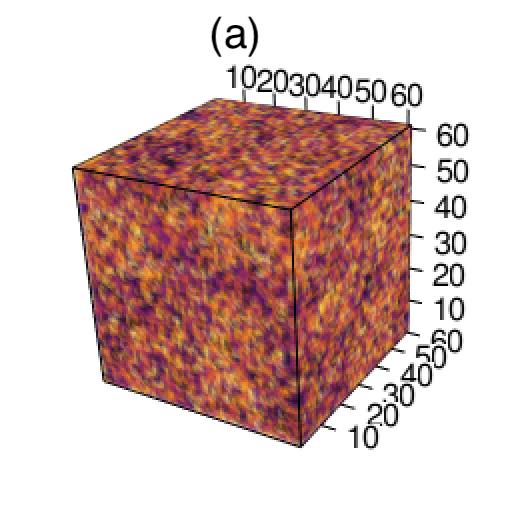
\includegraphics[scale=0.35]{figures/figure1/input.png}
	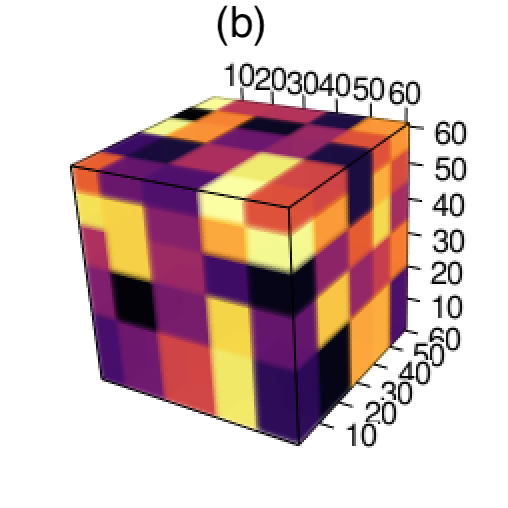
\includegraphics[scale=0.35]{figures/figure1/truth.png}
	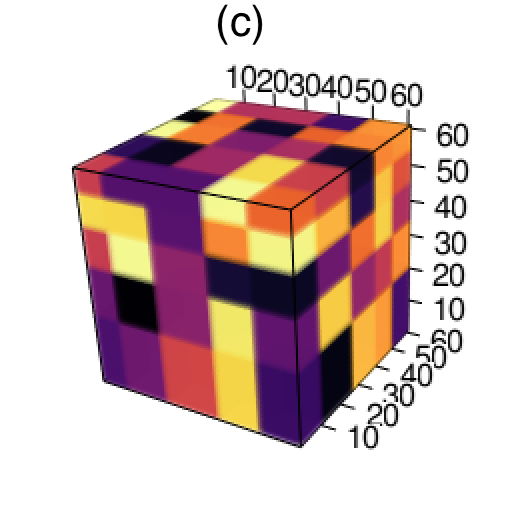
\includegraphics[scale=0.35]{figures/figure1/output.png}
	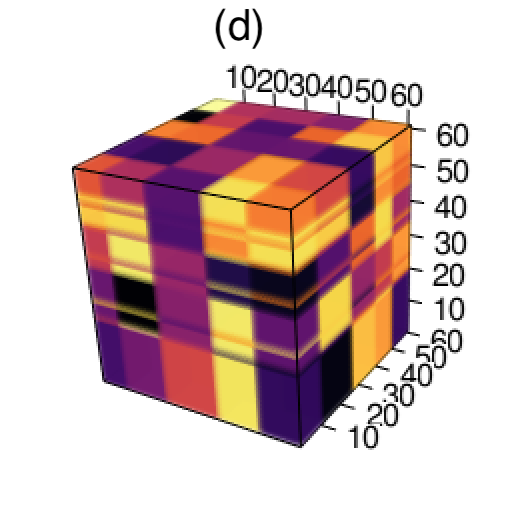
\includegraphics[scale=0.35]{figures/figure1/k_means.png}
	\caption{(a): a $60\times 60\times 60$ tensor with 5 clusters in each mode; (b): true underlying mean signal within each cluster; (c): mean signal estimated by our proposed approach with true number of clusters (5, 5, 5); (d): mean signal estimated by k-means clustering on each mode with true number of clusters (5 , 5, 5).}
	\label{fig:1}
\end{figure}

%\begin{figure}
%	\centering
%	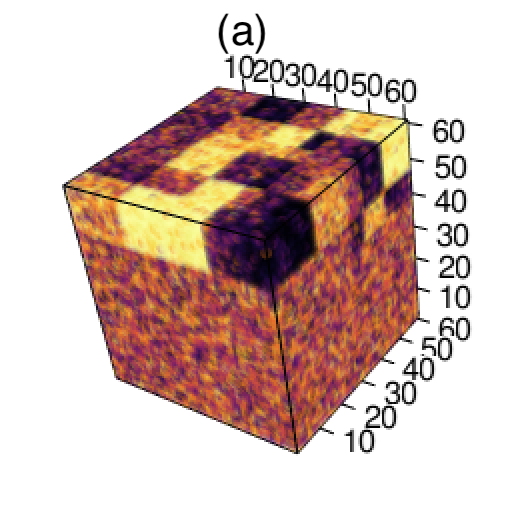
\includegraphics[scale=0.5]{figures/figure2/input.png}
%	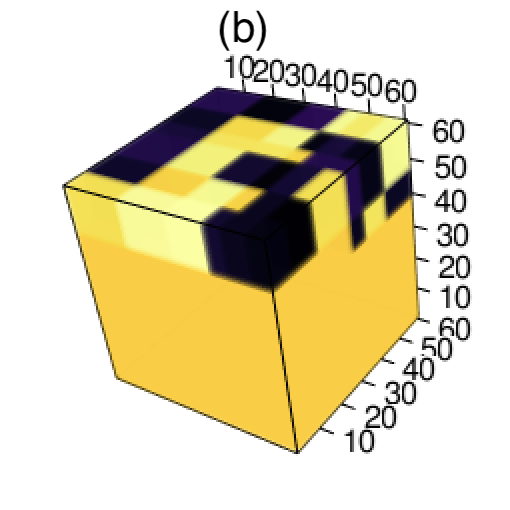
\includegraphics[scale=0.5]{figures/figure2/truth.png}
%	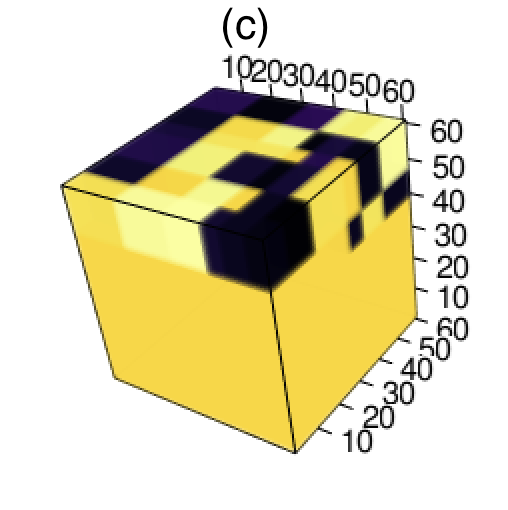
\includegraphics[scale=0.5]{figures/figure2/output.png}
%	\caption{(a): $60\times 60\times 60$ sparse tensor; (b) true underlying means; (c) mean signal estimated by our approach with estimated number of clusters and estimated $\lambda$.}
%	\label{fig:2}
%\end{figure}


\section{Preliminaries}

We say that an event $A$ occurs ``with high probability'' if $\mathbb{P}(\mA)$ tends to 1 as the dimension $d_{\min}=\min\{d_1,\ldots,d_k\}$ tends to infinity. We say that $A$ occurs ``with very high probability'' if $\mathbb{P}(A)$ tends to 1 faster than any polynomial of $d$. 


We use lower-case letters ($a,b,u,v,\ldots$) for scalars and vectors. We use upper-case boldface letters ($\mA,\mB,\mC,\ldots$) for matrices, and calligraphy letter ($\tA, \tB, \tC,\ldots$) for tensors of order $K\geq 3$. $\mx\otimes \my$ is the Kronecker product of two vectors. For any set $J$, $|J|$ denotes its cardinality. $[d]$ represents the set $\{1,2,\ldots,d\}$. 

A clustering of $d$ objects can be represented by a partition of the index set $[d]=\{1,\ldots,d\}$ into $R$ disjoint non-empty subsets. We refer to $R$ the clustering size. It is often convenient to represent the clustering (or partition) using the ``membership matrix''. A membership matrix $\mM$ is an $d$-by-$R$ matrix whose $(i,j)$-entry is 1 if and only if the element $i$ belongs to the cluster $j$, and 0 otherwise. 
%Based on the definition, $\mM$ is binary matrix with orthogonal columns, and the matrix elements sum up to $d$. 
The membership matrix $\mM$ can also be viewed as a mapping $\mM:[d]\mapsto[R]$. With a little abuse of notation, we still use the $\mM$ to denote the mapping, and use $\mM(i)$ to denote the cluster label that entry $i$ belongs to. Throughout the paper, we will use the terms ``partition'', ``clustering'', and ``membership matrix'' exchangeably. 

For a higher-order tensor, the above concepts can be applied to each of the modes. We use the term ``cluster'' to refer to the partition along the $k$-th mode of the tensor, and reserve ``block'' for the multi-way block in the tensor. 

\section{Tensor block model}
Let $\tY=\entry{y_{i_1,\ldots,i_K}}\in\mathbb{R}^{d_1\times \cdots\times d_K}$ denote an order-$K$, $(d_1,\ldots,d_K)$-dimensional data tensor. The main assumption on tensor block model is that the observed data tensor $\tY$ is a noisy realization of an underlying tensor that exhibits a checkerbox structure (see Figure~\ref{fig:1}). Specifically, suppose that there are $R_k$ clusters along the $k$-th mode of the tensor for $k\in[K]$. If the tensor entry $y_{i_1,\ldots,i_K}$ belongs to the block jointly determined by the $r_k$-th mode-$k$ cluster with $r_k\in[R_k]$, then we assume that 
\begin{equation}\label{eq:model}
y_{i_1,\ldots,i_K}=c_{r_1,\ldots,r_K}+\varepsilon_{i_1,\ldots,i_K},\quad \text{for }(i_1,\ldots,i_K)\in[d_1]\times\cdots\times [d_K],
\end{equation}
where $\mu_{r_1,\ldots,r_K}$ is the mean of the tensor block indexed by $(r_1,\ldots,r_K)$, and $\varepsilon_{i_1,\ldots,i_K}$'s are independent, mean-zero noise terms to be specified later. Our goal is to (i) find partitions along each of the modes, and (ii) estimate the block means $\{c_{r_1,\ldots,r_K}\}$, such that a corresponding blockwise-constant checkerbox structure emerges in the data tensor. 

The above tensor block model~\eqref{eq:model} falls into a larger class of non-overlapping, constant-mean clustering models~\cite{madeira2004biclustering}, in that each tensor entry belongs to exactly one block with a common mean. The model~\eqref{eq:model} can be equivalently expressed as a special tensor Tucker model,
\begin{equation}\label{eq:Tucker}
\tY=\tC\times_1\mM_1\times_2\cdots \times_K \mM_K+\tE,
\end{equation}
where $\tC\in\mathbb{R}^{R_1\times\cdots\times R_K}$ is a core tensor consisting of block means, $\mM_k \in\{0,1\}^{R_k\times d_k}$ are membership matrices indicating the block allocations along mode $k$ for $k\in[K]$, and $\tE=\entry{\varepsilon_{i_1,\ldots,i_K}}$ is the noise tensor. The distinction between our model~\eqref{eq:Tucker} and a classical Tucker model is that we require the factors $\mM_k$ to be membership matrices. Our model~\eqref{eq:Tucker} can be viewed as a super-sparse Tucker model, in the sense that the each column of $\mM_k$ consists of one copy of 1's and massive 0's. 

We now introduce the assumptions on the noise tensor $\tE$. We assume that $\varepsilon_{i_1,\ldots,i_K}$'s are independent, mean-zero, $\sigma$-subgaussian noises, where $\sigma>0$ is the subgaussianity parameter. More precisely, 
\begin{equation}\label{eq:noise}
\mathbb{E}e^{\lambda \varepsilon_{i_1,\ldots,i_K}}\leq e^{\lambda^2\sigma^2/2},\quad \text{for all } (i_1,\ldots,i_K)\in[d_1]\times\cdots\times[d_K] \ \text{and}\ \lambda\in\mathbb{R}.
\end{equation}
Th assumption~\eqref{eq:noise} is fairly general, which includes many common noises, such as Gaussian errors, Bernoulli errors, bounded errors, or even combinations of them. In particular, we consider two examples of the tensor block model that commonly appear in the literature:
\begin{exam}[Gaussian Multi-Cluster Model]
Let $\tY$ be a continuous-valued tensor. The Gaussian Multi-cluster model $y_{i_1,\ldots,i_K}  \sim_{\text{i.i.d.}} N(\mu_{r_1,\ldots,r_K},\sigma^2)$ is a special case of model~\eqref{eq:model} with the subgaussianity parameter $\sigma$ equal to the error variance.
\end{exam}

\begin{exam}[Stochastic Block Model]
Let $\tY$ be a binary-valued tensor. The multiway stochastic block model $y_{i_1,\ldots,i_K}  \sim_{\text{i.i.d.}} \text{Bernoulli}(\mu_{r_1,\ldots,r_K})$ is a special case of model~\eqref{eq:model} with the subgaussianity parameter $\sigma$ equal to ${1\over 4}$.
\end{exam}

More generally, our model also applied to hybrid error distributions in which different types of distribution can be allowed for different portions of the data. This scenario may happen, for example, when the data tensor $\tY$ represents concatenated measurements from multiple data sources. 


We consider a least-square approach for estimating model~\eqref{eq:model}. Let $\Theta=\tC\times_1\mM_1\times_2\cdots\times_K\mM_K$ denote the mean signal tensor with block structure. The mean tensor is assumed to belong to the following parameter space
\begin{align}\label{eq:space}
\tP_{R_1,\ldots,R_K}=&\ \big\{ \Theta\in\mathbb{R}^{d_1\times \cdots \times d_K}\colon \Theta=\tC\times_1\mM_1\times_2\cdots\times_K\mM_K, \text{with some}\\
 &\quad \text{membership matrices $\mM_k$'s and a core tensor $\tC\in\mathbb{R}^{R_1\times \cdots \times R_K}$}\big\}.
\end{align}
As in most previous work on tensor clustering, we assume that clustering size $\mR=(R_1,\ldots,R_K)$ are known in our theoretical analysis and simply write $\tP$ for short. In practice, $\mR$ needs to be determined from data; we address this general case in Section~\ref{sec:tuning}. The least-square estimator for model~\eqref{eq:model} is
\begin{equation}\label{eq:estimate}
\hat \Theta=\argmin_{\Theta\in\tP}\left\{ -2\langle \tY,\Theta\rangle + \FnormSize{}{\Theta}^2\right\}.
\end{equation}
The objective is equal (ignoring constants) to the sum of squares $\FnormSize{}{\tY-\Theta}^2$ and hence the name of our estimator. Estimating $\Theta$ consists of finding both the core tensor $\tC$ and the membership matrix estimates $\mM_k$'s. Before we discuss the properties of $\hat \Theta$, we present the identifiability of $\mM_k$'s and $\tC$ from $\Theta$. 

The following irreducible assumption is necessary for the tensor block model to be identifiable. 
\begin{ass}[Irreducible cores]\label{ass:core}
The core tensor $\tC$ is called irreducible if it cannot be written as a block tensor with the number of mode-$k$ clusters smaller than $R_k$, for any $k\in[K]$. 
\end{ass}
In the matrix case $(K=2)$, the assumption is equivalent to saying that $\tC$ has no two identical rows and no two identical columns. In the higher-order case, it requires that none of order-($K$-$1$) fibers of $\tC$ are identical. Note that the being irreducible is a weaker assumption than being full rank. 

\begin{prop}[Identifiability]\label{prop:factors}
Consider a Gaussian or Bernoulli tensor block model~\eqref{eq:Tucker}. Suppose the core tensor satisfies Assumption~\ref{ass:core}. Then every factor matrix $\mM_k$ is identifiable up to permutations of cluster labels. 
\end{prop}

Our identifiability result is stronger than the classical Tucker model. In a classical Tucker model~\cite{zhang2018tensor,kolda2009tensor} and many other factor analyses~\cite{darton1980rotation,abdi2003factor}, the factors are identifiable only up to orthogonal rotations. In those models, the (column) space spanned by $\mM_k$ can be recovered, but not the individual factors. In contrast, our model does not suffer from rotational invariance, and as we show in Section~\ref{sec:theory}, every single factor can be consistently estimated in high dimensions. This brings a benefit to the interpretation of tensor factors in the block model.  

%Finally, the permutation-invariance allows us to choose an ordering of indices for better visualization. The checkerbox pattern in Figure~\eqref{fig:1} thus should be interpreted as the estimate module some reordering along each of the modes. One can rearrange the indices in each mode to make the blocks contiguous; this amounts to multiplying $\mM_k$ by a permutation matrix $\mP_k\in\{0,1\}^{d_k\times d_k}$ and adjusting the core tensor $\tC$ by $\mP_k^{-1}$ accordingly. 


\section{Statistical convergence}\label{sec:theory}
In this section, we assess the estimation accuracy of the least-squares estimator~\eqref{eq:estimate}. The estimation accuracy is assessed using mean squared error (MSE):
\begin{equation}\label{eq:MSE}
\text{MSE}(\trueT,\hat \Theta)={1\over \prod_k d_k}\FnormSize{}{\trueT-\hat \Theta}^2,
\end{equation}
where $\trueT\in\tP$ is the true mean tensor and $\hat \Theta\in\tP$ is the estimator. 

While the least squares corresponds to the maximum likelihood estimator (MLE) for Gaussian tensor model, the same assertion does not hold for the other types of distribution such as stochastic tensor block model. Surprisingly, we will show that, with very high probability, a simple least-square estimator can achieve a nearly optimal convergence rate in a general class of block tensor models.  


\begin{theorem}[Convergence rate] \label{thm:main}
Let $\hat \Theta$ be the least-square estimator of $\trueT$ under model~\eqref{eq:model}. There exist two constants $C_1, C_2>0$ such that, with very high probability,  
\begin{equation}\label{eq:bound}
\text{MSE}(\trueT,\hat \Theta)\leq {C_1 \sigma^2\over  \prod_k d_k} \left(\prod_k R_k+\sum_k d_k \log R_k\right),
\end{equation}
holds uniformly over $\trueT\in\tP_{\mR}$ and all error distribution satisfying~\eqref{eq:noise}. 
\end{theorem}

The convergence rate in~\eqref{eq:bound} consists of two parts. The first part $\prod_k R_k$ reflects the complexity for estimating the core tensor $\tC$, while the second part $\sum_k d_k \log R_k$ results from the complexity for estimating the supports of $\mM_k$'s. It is the price that one has to pay for not knowing the locations of the blocks.  

We now compare our bound with existing literature. The classical Tucker tensor decomposition has a minimax convergence rate $\sum_kd_kR'_k$~\cite{zhang2018tensor}, where $R'_k$ is the multilinear rank at mode $k$. In the case of block model, this yields $\sum_kd_kR_k$, because the mode-$k$ rank is bounded by the number of clusters in mode-$k$. Now, as both the dimension $d_{\min}=\min_kd_k$ and clustering size $R_{\min}=\min_k R_k$ tend to infinity, we have $\prod_k R_k+ \sum_k d_k \log R_k\ll \sum_k d_k R_k$. Therefore, by fully exploiting the block structure, we obtain a better convergence rate than previously possible. 

Our bound generalizes the previous results on structured matrix estimation in network analysis~\cite{gao2016optimal,gao2018minimax}. The optimal convergence rate for estimating the (matrix) stochastic block model was $R_1R_2+d_1\log R_1+d_2\log R_2$~\cite{gao2016optimal}, which fits into our special case when $K=2$. 
Earlier work~\cite{gao2018minimax} suggests the following heuristics on the sample complexity for high-dimensional matrix problems:
\begin{equation}\label{eq:intuition}
{\text{(number of parameters)}+ \log \text{(complexity of models)}\over \text{number of samples}}.
\end{equation}
Our result supports this important principle for general $K\geq 2$. Note that, in tensor estimation, the total number of entries corresponds to the sample size $\prod_k d_k$, the number of parameters is $\prod_k R_k$, and combinatoric complexity for estimating block models is of order $\prod_k R_k^{d_k}$. The principle~\eqref{eq:intuition} thus provide an intuition for~\eqref{eq:bound}. 

%The optimality of the least-square estimator is safeguarded by the following information-theoretical lower bound.
%\begin{theorem}[Information-theoretical bound] Under the Gaussian or Bernoulli tensor block models, there exist some constants $\alpha_0>0, \beta_0\in(0,1)$, such that
%\[
%\inf_{\hat \Theta}\sup_{\Theta \in \tP}\mathbb{P}\left\{ \FnormSize{}{\hat \Theta-\trueT}^2> c_0\sigma^2 \prod_k R_k+\sum d_k \log R_k\right\}>\beta_0.
%\]
%(add the proof)
%\end{theorem}

We next study the clustering consistency of our method. Let $\mA_k, \mB_k$ be the two membership matrices along mode-$k$. We define the misclassification rate as $\text{MCR}(\mA_k,\mB_k)=d_k^{-1}\sum_{i\in[d_k]}\mathds{1}_{\{\hat \mA_k(i)=\mB_k(i)\}}$. The following Theorem implies that our method achieves clustering consistency. 

\begin{theorem}[Clustering consistency]\label{thm:partition}
Suppose the Assumption~\eqref{ass:core} holds. Let $\hat \mM_k$'s be the estimators from~\eqref{eq:estimate}. Then the proportions of misclassified indices goes to zero in probability; i.e. there exist permutation matrices $\mP_k$'s such that
\[
\sum_k \text{MCR}(\hat \mM_k, \mP_k\trueM) \rightarrow 0, \quad \text{in probability},
\]
\end{theorem}
(add the proof)
Under stronger distribution assumptions on $\tE$, we can establish the finite-sample convergence rate for the clustering accuracy. See more results in the Supplements. 

\section{Numerical Implementation}
\subsection{Alternating optimization}
We introduce an alternating optimization for solving~\eqref{eq:estimate}. Note that the optimization~\eqref{eq:estimate} can be written as
\begin{align}\label{eq:op}
(\hat \tC, \{\hat \mM_k\})&=\argmin_{\tC\in\mathbb{R}^{R_1\times \cdots \times R_K}, \text{ membership matrices $\mM_k$'s}} f(\tC,\{\mM_k\}),\notag\\
 \text{where}&\quad f(\tC,\{\mM_k\})=\FnormSize{}{\tY-\tC\times_1\mM_1\times_2\ldots\times_K\mM_K}^2.\notag
\end{align}
The decision variables consists of $K+1$ blocks of variables, one for the core tensor $\tC$ and $K$ for the membership matrices $\mM_k$'s. We notice that, if any $K$ out of the $K+1$ blocks of variables are known, then the last block of variables can be solved explicitly. This observation suggests that we can iteratively update one block of variables at a time while keeping other others fixed. Specifically, given the collection of $\hat \mM_k$'s, the core tensor estimate $\hat \tC=\argmin_{\tC}f(\tC,\{\hat \mM_k\})$ collects the sample averages within each tensor block. Given the block mean $\hat \tC$ and $K-1$ membership matrices, the last membership matrix can be solved using simple nearest neighbor search over only $R_k$ discrete points. The full procedure is described in Algorithm~\ref{alg:B}.

\begin{algorithm}
\caption{Multiway clustering based on tensor block models}\label{alg:B}
\begin{algorithmic}[1]
\INPUT Data tensor $\tY\in \mathbb{R}^{d_1\times \cdots \times d_K}$, clustering size $\mR=(R_1,\ldots,R_K)$.
\OUTPUT Block mean tensor $\hat \tC\in\mathbb{R}^{R_1\times \cdots\times R_K}$, and the membership matrices $\hat \mM_k$. 
\State Initialize the marginal clustering by performing independent $k$-means on each of the $K$ modes.
\Repeat
\State Update the core tensor $\hat \tC=\entry{\hat c_{r_1,\ldots,r_K}}$. Specifically, for each $(r_1,\ldots,r_K)\in[R_1]\times \cdots [R_K]$,
\begin{equation}\label{eq:ols}
\hat c_{r_1,\ldots,r_K}={1\over n_{r_1,\ldots,r_K}}\sum_{\hat \mM_1^{-1}(r_1)\times\cdots\times \hat \mM_K^{-1}(r_K)}{\tY_{i_1,\ldots,i_K}},
\end{equation}
where $n_{r_1,\ldots,r_K}=\prod_k|\hat \mM_k^{-1}(r_k)|$ is the number of entries in the block indexed by $(r_1,\ldots,r_K)$. 
\State Update membership matrices $\hat \mM_k$'s:
\For{$k$ in $\{1,2,...,K\}$}
\State Update the mode-$k$ membership matrix $\hat \mM_k$. Specifically, for each $a\in[d_k]$, assign the cluster label $\hat \mM_k(a)\in[R_k]$ for which	\[
\hat \mM_k(a)=\argmin_{r\in[R_K]}\sum_{\mI_{-k}}\left(c_{\hat \mM_1(i_1),\ldots,r,\ldots,\hat \mM_K(i_K)}-\tY_{i_1,\ldots,a,\ldots,i_K}\right)^2,
\]
where $\mI_{-k}=(i_1,\ldots,i_{k-1},i_{k+1},\ldots,i_K)$ denotes the coordinates except the $k$-th mode. 
\EndFor
\Until{Convergence} 
\end{algorithmic}
\end{algorithm}
The above algorithm can be viewed as a higher-order extension for the ordinary (one-way) $k$-means algorithm. The core tensor $\tC$ serves as the role of centroids. As each iteration reduces the value of the objective function, which is bounded below, convergence of the algorithm is guaranteed. On the other hand, obtaining the global optimizer for such a non-convex optimization is typically difficult, even for the one-way $k$-means~\cite{aloise2009np}. As such, we run the algorithm multiple times, using random initializations of the independent one-way $k$-mean on each of the $K$ modes. 

\subsection{Tuning parameter selection}\label{sec:tuning}
Our algorithm~\ref{alg:B} takes the number of clusters $\mR$ as an input. In practice such information is often unknown and $\mR$ needs to be estimated from the data $\tY$. We propose to select this tuning parameter using Bayesian information criterion (BIC), 
\begin{equation}\label{eq:BIC}
\text{BIC}(\mR) =  \log\left(\FnormSize{}{\tY-\hat \Theta}^2\right)+{ \sum_k \log d_k \over \prod_k d_k}p_e,
\end{equation}
where $p_e$ is the effective number of parameters in the model. In our case we take $p_e=\prod_k R_k+\sum_k d_k\log R_k$, which is inspired from~\eqref{eq:intuition}. We choose $\hat \mR$ that minimizes $\text{BIC}(\mR)$ via grid search. Our choice of BIC is based on heretics, and we test its empirical performance in Section~\ref{sec:simulation}.  

\section{Extension to regularized estimation}
In some large-scale applications, not every block in a data tensor is of equally importance. Examples include genome expression data, in which only a few entries represent the signals while the majority comes from the background noise (see Figure~\ref{fig:2}). Another example is community detection in a large sparse network, where only a few blocks represent the communities of interest and others represent small, noisy groups with weak connection.  Although our estimator~\eqref{eq:estimate} can still handle this scenario by assigning small value to some of the $\hat c_{r_1,\ldots,r_K}$'s, the estimates may suffer from high variance. It is thus beneficial to introduce regularized estimation for better bias-variance trade-off and improved interpretability. 

Here we illustrate the regularized estimation using \emph{sparsity} on the block means for localizing important blocks in the data tensor. This problem can be cast into variable selection on the block parameters. We propose the following regularized least-square estimation:
\[
\hat \Theta^{\text{sparse}}=\argmin_{\Theta\in \tP}\left\{\FnormSize{}{\tY-\Theta}^2+\lambda \normSize{}{\tC}_\rho
\right\},
\]
where $\normSize{}{\tC}_\rho$ is the penalty function with $\rho$ being an index for the tensor norm, $\tC\in\mathbb{R}^{R_1\times \cdots\times R_K}$ is the block means, and $\lambda$ is the penalty tuning parameter. Some widely used penalties include Lasso penalty $(\rho=1)$, sparse subset penalty $(\rho=0)$, ridge penalty $(\rho=\text{Frobenius norm})$, elastic net (linear combination of $\rho=1$ and $\rho=\text{Frobenius norm}$), among many others. 

For parsimony purpose, we only discuss the properties for Lasso and sparse subset penalties here; other penalizations can be derived similarly. Sparse estimation incurs slight changes to Algorithm~\ref{alg:B}. When updating the core tensor $\tC$ in~\eqref{eq:ols}, we fit a penalized least square problem with respect to $\tC$. 
%\[
%\hat \tC^{\text{sparse}}=\argmin_{\tC\in\mathbb{R}^{R_1\times \cdots\times R_K}} \FnormSize{}{\tY-\tC\times_1\hat \mM_1\times\cdots\times_K \hat \mM_K}^2+\lambda \normSize{}{\tC}_\rho.
%\]
The closed form for the entry-wise sparse estimate $\hat c^{\text{sparse}}_{r_1,\ldots,r_K}$ is (See Lemma~\ref{lem:sparse} in Appendix):
\begin{equation}\label{eq:lasso}
\hat c^{\text{sparse}}_{r_1,\ldots,r_K}=
\begin{cases}
\hat c^{\text{ols}}_{r_1,\ldots,r_K}\mathds{1}_{\{|\hat c^{\text{ols}}_{r_1,\ldots,r_K} |\geq {2\sqrt{\lambda} \over \sqrt{n_{r_1,\ldots,r_K}}}\}} & \text{if}\ \rho=1,\\
\text{sign}(\hat c^{\text{ols}}_{r_1,\ldots,r_K})\left( \hat c^{\text{ols}}_{r_1,\ldots,r_K}-{2\lambda \over n_{r_1,\ldots,r_K}}  \right) &\text{if}\ \rho=0.
\end{cases}
\end{equation}
where $\hat c^{\text{ols}}_{r_1,\ldots,r_K}$ denotes the ordinary least-square estimate in~\eqref{eq:ols}, for all $(r_1,\ldots,r_K)\in[d_1]\times\cdots[d_K]$. 
%From Equation~\eqref{eq:lasso}, we note that the penalization on $\tC$ shrink some block means to zero, and the shrinkage depends on the block size. For two blocks with same mean $\hat c^{\text{ols}}_{r_1,\ldots,r_K}$, the smaller block receives a more stringent thresholding value $\lambda/ n_{r_1,\ldots,r_K}$. As such, our penalization results in sparse estimates of the block means, and it is useful for detecting important blocks from a large data tensor. 
The choice of penalty function $\rho$ often depends on the goals and interpretations in specific applications. Given a penalization, we choose to select the tuning parameter $\lambda$ via BIC~\eqref{eq:BIC}, where we modify $p_e$ into $p^{\text{sparse}}_e=\normSize{}{\hat \tC^{\text{sparse}}}_0+\sum_kd_k\log R_k$, where $\normSize{}{\cdot}_0$ denotes the number of non-zero entries in the tensor. The empirical performance of this proposal will be evaluated in Section~\ref{sec:simulation}. 



\section{Experiments}\label{sec:simulation}
In this section, we evaluate the empirical performance of our method. We consider both non-sparse and sparse tensors, and compare the recovery accuracy with other tensor-based methods. 

%For sparsity tensor, we further consider the following three statistics:
%(3) Total Correct Rate: 1 - the proportion of misjudgment while determining whether the mean signal is zero.;\\
%(4) Correct Zero Rate: the proportion of zero elements are correctly identified in the underlying mean tensor;\\

\subsection{Finite-sample performance}

We generate noisy order-3 tensors under the tensor block model~\eqref{eq:model}. We consider various values of dimension $\md=(d_1,d_2,d_3)$ and clustering size $\mR=(R_1,R_2,R_3)$ as we described below. Along each mode, the tensor entries are randomly assigned into clusters with uniform probability. The block means are generated i.i.d.\ from Unif[-3,3]. The entries in the noise tensor $\tE$ are generated from i.i.d.\ Gaussian $(0,\sigma^2)$. In each simulation study, we report the summary statistics across $n_{\text{sim}}=50$ replications. 

\begin{figure}[http]
\centering
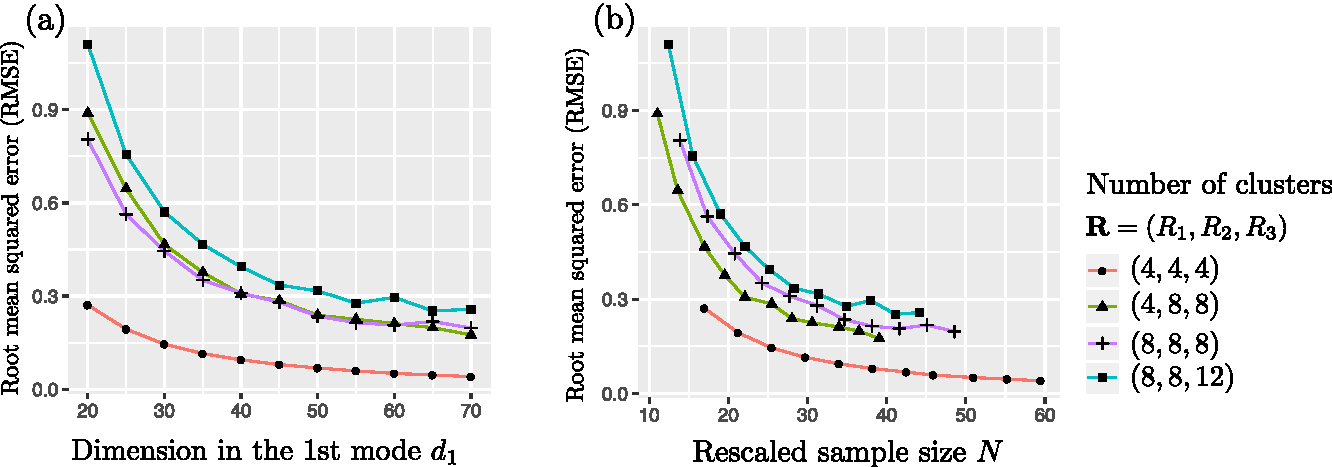
\includegraphics[width=1\textwidth]{figures/figure3/decay.pdf}
\caption{Estimation error for block tensors with Gaussian noise. Each curve corresponds to a fixed clustering size $\mR$. (a) Plot of average RMSE against $d_1$. (b) Plot of average RMSE against rescaled sample size $N=\sqrt{d_2d_3/\log R_1}$. 
}\label{fig:RMSE}
\end{figure}

In the first experiment, we assess the empirical relationship between the root mean squared error (RMSE) and the dimension. We set $\sigma=3$ and consider four different $\mR$ settings (see Figure~\ref{fig:RMSE}). We increases $d_1$ from 20 to 70, and for each choice of $d_1$, we set the other two dimensions $(d_2,d_3)$ such that $d_1\log R_1\approx d_2\log R_2\approx d_3\log R_3$. Our theoretical analysis suggests that the RMSE converges at least at the rate of $\sqrt{\log R_1/d_2d_3}$ in this case. Figure~\ref{fig:RMSE}a plots the recovery error versus the dimension $d_1$. We rescaled the x-axis in Figure~\ref{fig:RMSE}b, and find that RMSE decreases roughly at the rate of $1/N$, where $N=\sqrt{d_2d_3/\log R_1}$ is the rescaled sample size. This is consistent to our theoretical result. It is observed that tensors with a higher number of blocks tend to yield higher recovery errors, as reflected by the upward shift of the curves as $\mR$ increases. Indeed, a higher $\mR$ means a higher intrinsic dimension of the problem, thus increasing the difficulty of the estimation. 

In the second experiment, we evaluate the selection performance of our BIC criterion~\eqref{eq:BIC}. Supplementary Table 1 reports the selected numbers of clusters various combinations of dimension $\md$, clustering size $\mR$, and noise $\sigma$. We find that, for the case $\md=(40,40,40)$ and $\mR=(4,4,4)$, the BIC selection is accurate in the low-to-moderate noise setting. In the case of high noise $\sigma=12$, the 
selected number of clusters is slightly smaller than the true number, but the accuracy increases when either the dimension increases to $\md=(40,40,80)$ or the clustering size reduces to $\mR=(2,3,4)$. Within a tensor, the selection seems to be easier for shorter modes with smaller number of clusters, and this is to be expected, since shorter mode has more effective samples for clustering. 


\subsection{Comparison with alternative methods}
Next, we compare our method with two popular low-rank tensor estimation methods: (i) CP decomposition and (ii) Tucker decomposition. The CP model decomposes a tensor into a sum of rank-1 tensors, whereas Tucker model decomposes a tensor into a core tensor multiplied by orthogonal matrices in each mode. Following the literature~\cite{chi2018provable}, we perform the clustering by applying the $k$-means to the resulting factors along each of the modes. We refer to such techniques as CP+$k$-means and Tucker+$k$-means. 

\begin{figure}
	\centering
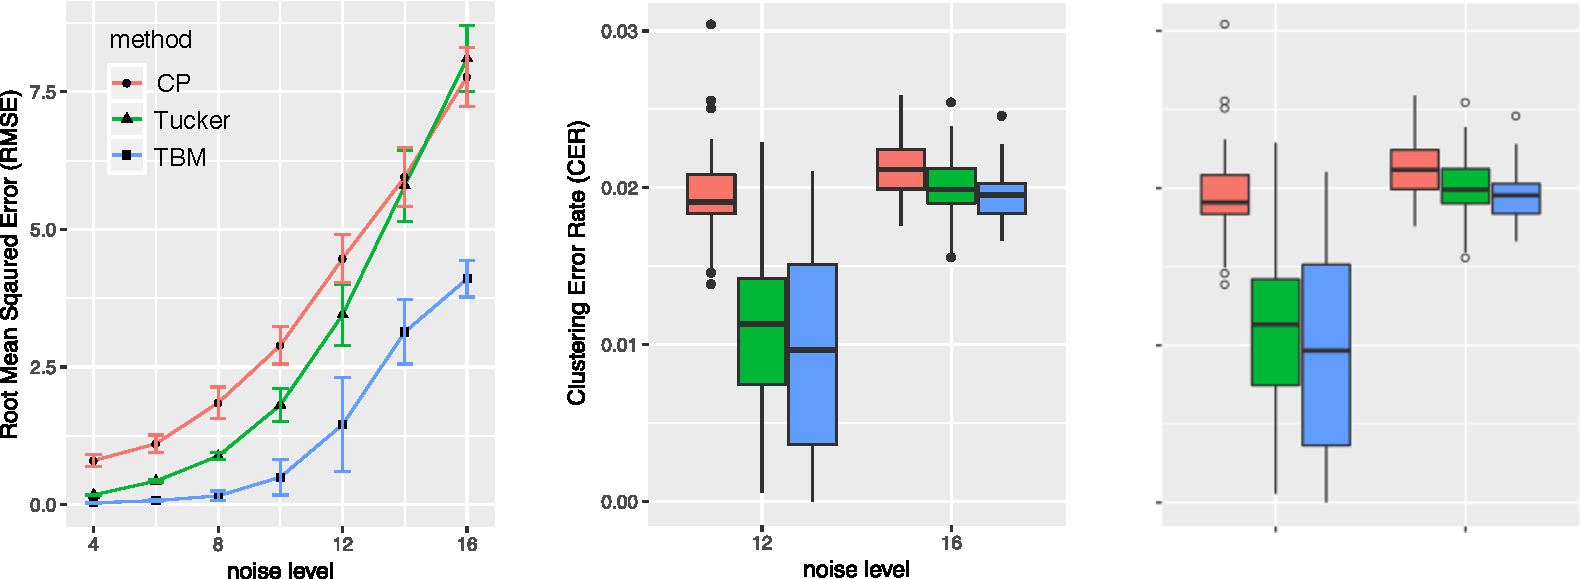
\includegraphics[width=\textwidth]{figures/test}
	\caption{Performance comparison in terms of RMSE and CER. (a) Plot of the estimation error against noise. (b) Boxplot of the clustering error against noise for tensors of dimension $(40,40,40)$. (c) Boxplot of the clustering error against noise for tensors of dimension $(60,60,60)$.} \label{fig4}
\end{figure}

For easy reference, we denote our method by TBM (tensor block model)\footnote{TBM implementation: https://github.com/wanglab/tensorsparse}. We generate noisy block tensors with 5 clusters on each of the modes, and then assess both the estimation and clustering performance for each method. Note that our method takes a single step to perform estimation and clustering simultaneously, whereas the CP and Tucker-based approaches take a two-step procedure. We use the RMSE to assess the estimation accuracy and use the clustering error rate (CER) to measure the clustering accuracy. The CER is calculated using the disagreements (i.e., one minus rand index) between the true and estimated block partitions in the three-way data. For fair comparison, we provide all methods the true number of clusters. 

Figure~\ref{fig4} compares the performance. We find that TBM achieves the lowest estimation error among the three methods. The gain in accuracy is more pronounced as the noise grows. Both CP and Tucker fail to accurately estimate the signal tensor, but Tucker appears to have a modest clustering performance. One possible explanation is that Tucker enforces orthogonality in the factors which make the subsequent $k$-means clustering easier. Figure~\ref{fig4} shows that the clustering error increases with noise but decreases with dimension. This agrees with our expectation, as in tensorial data analysis, a larger dimension implies a larger sample size. 



\textbf{Sparse case.} We then assess the performance when the signal tensor is sparse. We modify the generation of block means using a mixture distribution of zero mass and Unif[-3,3], with probability $p$ and $1-p$ respectively. The $p$ is called the sparsity rate. We generate noisy tensors of dimension $\md=(40,40,40)$ with varying levels of sparsity and noise. The initial clustering size is set $\mR=(3,4,5)$, but the actual number of clusters may be smaller because zero-mean blocks could be merged together. We primarily focus on the estimation and selection accuracy. The selection accuracy is quantified via the the sparsity error rate, which is the proportion of entries that were incorrectly set to zero or incorrectly set to non-zero. We also report the proportion of true zero's that were correctly identified (correct zeros). 

We utilize $\ell0$-penalized TBM and select the sparse parameter $\lambda$ via BIC. Table~\ref{t5} reports the selected $\lambda$ averaged across 50 simulations. We see a substantial benefit obtained by penalization. Our proposed $\lambda$ is able to guide the algorithm to correctly identify zero's while maintaining good accuracy in identifying non-zero's. The resulting sparsity level is close to the ground truth. The rows with $\lambda=0$ correspond to the three non-sparse algorithms (CP, Tucker, and non-sparse TBM). Because non-sparse algorithms fail to identify zero's, they show equally poor performance in all metrics. Supplementary Figure~\ref{} shows the the estimation error in terms of RMSE. Again, the sparse TBM outer-performs the other two methods. 

\begin{table}[http]
	 \resizebox{1\textwidth}{!}{%
	\begin{tabular}{|c|c|c|c|c|c|}
		\hline
		Sparsity ($\rho$)&Noise $(\sigma)$&Penalization $(\lambda)$&Estimated Sparsity Rate&Correct Zero Rate&Sparsity Error Rate  \\ \hline
		\multirow{2}{*}{0.5}&\multirow{2}{*}{4}&$\lambda=0$&$0(0)$&$0(0)$&$0.49(0.07)$\\
		&&$\bar{\lambda}=86.6$&${\bf 0.56(0.07)}$&${\bf 0.99(0.01)}$&$\mathbf{0.07(0.04)}$\\
		\hline
		\multirow{2}{*}{0.5}&\multirow{2}{*}{8}&$\lambda=0$&0(0)&0(0)&$0.49(0.07)$\\
		&&$\bar{\lambda}=344.4$&${\bf 0.63(0.07)}$&${\bf 0.99(0.01)}$&$0.14(0.05)$\\
		\hline
		\multirow{2}{*}{0.8}&\multirow{2}{*}{8}&$\lambda=0$&$0(0)$&$0(0)$&$0.80(0.05)$\\
		&&$\bar{\lambda}=246.9$&${\bf 0.83(0.06)}$&${\bf 0.95(0.04)}$&${\bf 0.12(0.06)}$\\
		\hline
	\end{tabular}
	}
	\caption{Results for sparse tensor block estimation under dimension $\md=(40,40,40)$. The reported $\bar \lambda$ is the mean of $\lambda$ selected across 50 simulations using our proposed BIC criterion. Number in bold indicates no significant difference between the estimate and the ground truth, based on a $z$-test with a level 0.05.}\label{t5}
\end{table}

%\begin{figure}
%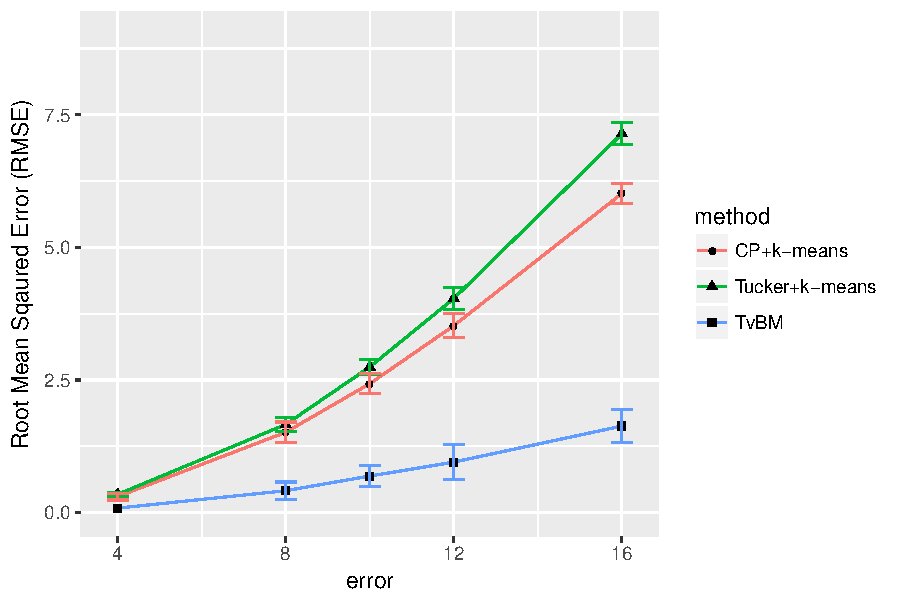
\includegraphics[width=.5\textwidth]{figures/sparse}
%\end{figure}

\section{Real data analysis}
Lastly, we applied our method on two real data sets, one is a real-valued tensor and another is a Bernoulli-valued tensor. The real-valued dataset consists of gene expressions from 13 brain tissues, 100 individuals, and 193 genes. The dataset is obtained from GTEx contortion, and the gene list comes from... We subtract the overall mean and apply the penalized TBM method on this tensor. Tensor blocks are identified. We select 10 blocks and . We find that tissues are collected.

Another dataset we consider is the \emph{Nations} data. The nations data set is a $14\times 14 \times 56$ binary tensor consisting of 56 political relationships of 14 countries between 1950 and 1965. There are 78.9\% of entries are zero. We applied the BIC criterion and choose $\mR=(5,5,9)$ and $\lambda=0.4$. 


\section{Conclusion}
Sparsity is only one form of regularization. In specific applications, prior knowledge often suggests various constraints among parameters, which may be exploited to regularize parameter estimates. For example, in the stochastic block model, sometimes it may be reasonable to impose symmetry on the parameters along certain subsets of modes, which further reduces the dimension of the problem. In some other applications, non-negativity of parameter of parameter values may be enforced. In our software, we implement the common penalizations but leave .. .to further study. 



\bibliographystyle{unsrt}
\bibliography{tensor_wang}


\end{document}
